\documentclass[border=10pt]{standalone}
\usepackage{pgfplots}
\pgfplotsset{compat=1.18}
\begin{document}
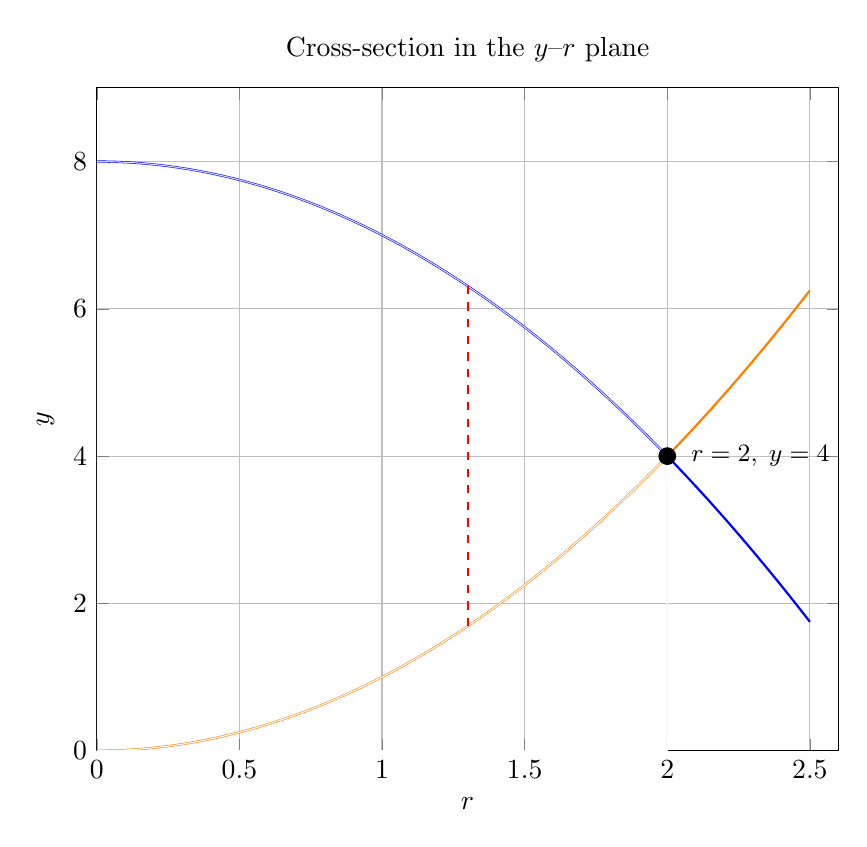
\begin{tikzpicture}
\begin{axis}[
    xlabel={$r$}, ylabel={$y$},
    xmin=0, xmax=2.6, ymin=0, ymax=9,
    title={Cross-section in the $y$--$r$ plane},
    width=11cm, height=10cm,
    grid=major,
]
% Curves
\addplot[blue, thick, domain=0:2.5, samples=80] {8 - x^2};
\addplot[orange, thick, domain=0:2.5, samples=80] {x^2};

% Filled region between curves on [0,2]
\addplot[blue!15, domain=0:2, samples=60] {8 - x^2} \closedcycle;
\addplot[white, domain=0:2, samples=60] {x^2} \closedcycle;

% Highlight typical washer at r=1.3
\addplot[red, dashed, thick] coordinates {(1.3, 1.69) (1.3, 6.31)};

% Intersection marker
\addplot[only marks, mark=*, mark size=3pt, black] coordinates {(2, 4)};
\node[font=\small, anchor=west] at (axis cs:2.05, 4) {$r=2,\;y=4$};
\end{axis}
\end{tikzpicture}
\end{document}